\chapter[Desenvolvimento do Produto]{Desenvolvimento do Produto}

\section[Ergonomia e Design]{Ergonomia e \textit{Design}}

Nesta seção, será apresentado o conceito e o funcionamento do produto com seus principais mecanismos, assim como os cálculos necessários para o dimensionamento dos seus componentes. Além disso, é apresentado uma análise ergonômica, que avalia o grau de conforto de variados perfis de usuários (homens, mulheres e idoso).

O conceito do produto é apresentado na figura \ref{conceito} na qual o sistema de coordenadas estabelecido serve de referência para todo o trabalho.


\begin{figure}[htb]
		\centering
			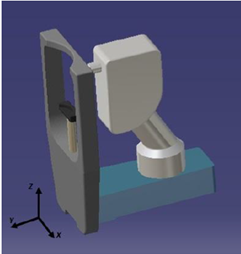
\includegraphics[scale=1.0]{figuras/conceito.png}
		\caption{Conceito em CAD do produto final}
		\label{conceito}
\end{figure}

\subsection[Metodologia de Desenvolvimento]{Metodologia de Desenvolvimento}

A metodologia de trabalho utilizada consistiu primeiramente em reconhecer os requisitos do equipamento. Desta forma, foi realizado um estudo sobre as possíveis soluções para as problemáticas encontradas e então escolheu-se aquela que satisfazia as condições desejadas. Neste sentido foi feito o delineamento do anteprojeto da máquina e o dimensionamento de seus componentes. Por conseguinte, foi realizado seus desenhos técnicos e especificações através do software CATIA.

A Figura \ref{met}, traz um diagrama que esquematiza as considerações levadas em conta ao realizar o projeto.

\begin{figure}[H]
		\centering
			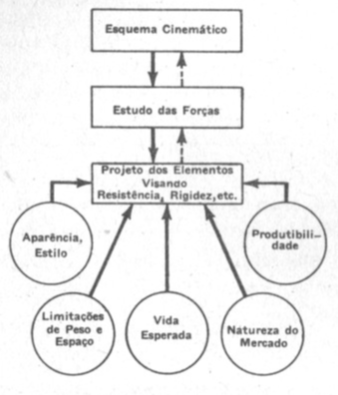
\includegraphics[scale=1.0]{figuras/met.png}
		\caption{Diagrama de Metodologia \cite{shigley}}
		\label{met}
\end{figure}

\subsection[Mecanismos de Movimentação]{Mecanismos de Movimentação}

Os mecanismos projetados nesse projeto possuem a finalidade de produzir movimentos nas três direções tomadas como referencia que foram apresentadas na figura \ref{conceito}. Todos os mecanismos têm como objetivo principal o movimento suave e seguro para que assim não ocorra o comprometimento da saúde do usuário.

\subsubsection[Mecanismo responsável pela movimentação em relação eixo x]{Mecanismo responsável pela movimentação em relação eixo x}

Engrenagens sem fim podem ser comparadas a um parafuso (eixo) e sua rosca (coroa). A Figura \ref{eng} apresenta um sistema de engrenagens sem fim, este tipo de engrenagem é uma variação das engrenagens helicoidais com a diferença de que o ângulo de hélice é muito grande, o que permite o contato continuo entre os dentes das engrenagens. Desta forma com este tipo de engrenagem é possível realizar movimentos de alta precisão, que é o caso deste trabalho \cite{norton}.

\begin{figure}[H]
		\centering
			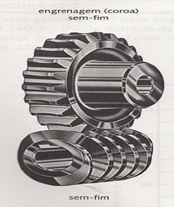
\includegraphics[scale=1.0]{figuras/eng.png}
		\caption{Exemplo de sistema de engrenagem sem fim \cite{norton}.}
		\label{eng}
\end{figure}

Para dimensionamento do sistema sem fim, Norton sugere uma rotina de cálculos em que a partir de parâmetros geométricos da coroa e do eixo sem fim, é calculado se o torque resultante no sistema é suficiente para movimentar a estrutura. Desta forma gerou-se uma rotina MatLab, disponível no Apêndice A, em que utilizou-se como dado de entrada dados referentes a componentes comerciais que foram testados segundo a lógica apresentada na figura \ref{fluxdi}. Diante disso, foi escolhido um conjunto comercial M8 para a haste com fuso.

\begin{figure}[htb]
		\centering
			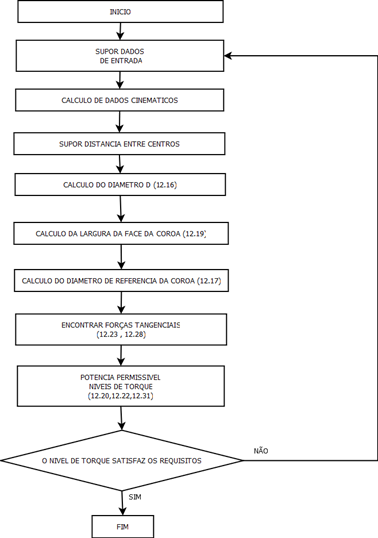
\includegraphics[scale=1.3]{figuras/fluxdi.png}
		\caption{Fluxograma para dimensionamento do sistema sem-fim}
		\label{fluxdi}
\end{figure}

A Figura \ref{eixox} mostra metade da estrutura responsável pela movimentação do produto no eixo “x”. Ela é composta por dois conjuntos em que cada um possui um motor de passo que aplica um torque sobre o eixo sem fim, que por sua vez é transmitido para a coroa, que se desloca axialmente, movendo a estrutura. Além disso, há também dois eixos secundários que dão estabilidade e resistência mecânica a estrutura.

\begin{figure}[H]
		\centering
			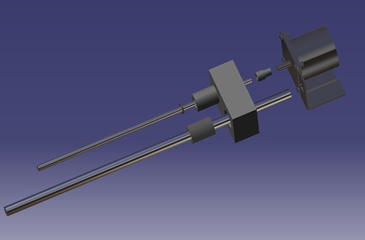
\includegraphics[scale=1.0]{figuras/eixox.png}
		\caption{Metade do mecanismo do eixo x}
		\label{eixox}
\end{figure}

O mecanismo completo pode ser visualizado na figura \ref{eixox2} em que é apresentado também uma representação de um usuário utilizando o equipamento. Além disso, a visualização do mecanismo de movimentação no interior do produto pode ser observada.

\begin{figure}[H]
		\centering
			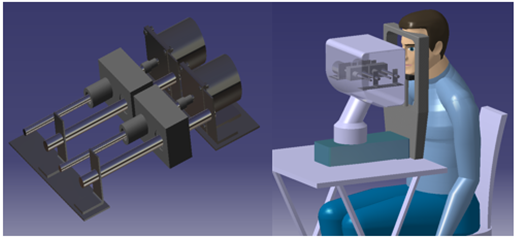
\includegraphics[scale=1.0]{figuras/eixox2.png}
		\caption{Mecanismo do eixo "x" completo}
		\label{eixox2}
\end{figure}

Na Figura \ref{eixox3}, é possível observar o mecanismo completo do eixo “x” em uma vista explodida, na qual todos os componentes são explicitados. Para sua montagem, foi utilizado vários componentes em modelos comerciais, como o motor de passo, as hastes, porcas e parafusos. O suporte para haste, será confeccionado em plástico pela impressora 3D. Além disso, os suportes para haste lisa, número 10, são de alumínio.

\begin{figure}[H]
		\centering
			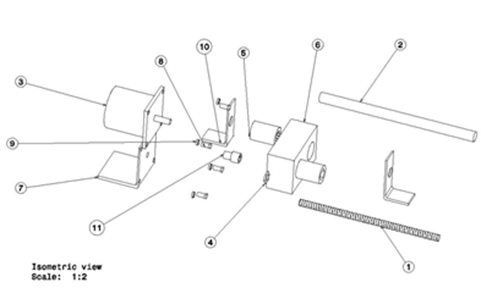
\includegraphics[scale=1.0]{figuras/eixox3.png}
		\caption{Componentes do mecanismo do eixo “x”}
		\label{eixox3}
\end{figure}

A figura \ref{eixox31}, traz a lista de todos os componentes citados na \ref{eixox3}.

\begin{figure}[H]
		\centering
			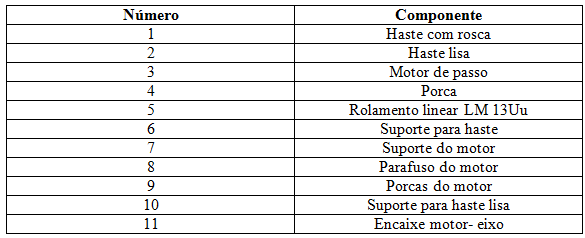
\includegraphics[scale=1.0]{figuras/eixox31.png}
		\caption{Lista de componentes apresentados na figura \ref{eixox3}}
		\label{eixox31}
\end{figure}

\subsubsection[Mecanismo responsável pela movimentação em relação eixo y]{Mecanismo responsável pela movimentação em relação eixo y}

O mecanismo referente ao movimento do eixo “y”, assim como no movimento em “x”, também utiliza um sistema de eixo sem fim acionado por um motor de passo. Desta forma, o modo como o mecanismo será dimensionado é semelhante.

Neste caso, utiliza-se como inspiração o sistema encontrado no micrômetro, cuja precisão é alta. A Figura \ref{micro} ilustra os mecanismos encontrados no micrômetro. O movimento neste tipo de mecanismo se dá quando o tambor é rotacionado. Ele possui acoplamento direto com a porca de ajuste que é solidária ao seu movimento. Quando a porca de ajuste gira, desloca o parafuso para frente ou para trás. Neste caso somente será utilizado o cabeçote do micrômetro, dispensando o arco, o protetor antitérmico e o fixador.

\begin{figure}[H]
		\centering
			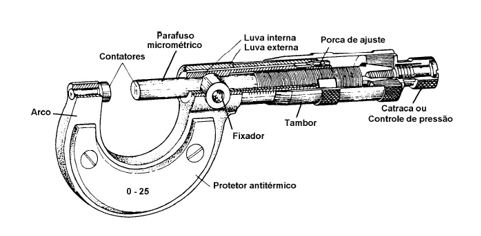
\includegraphics[scale=1.0]{figuras/micro.png}
		\caption{Micrômetro}
		\label{micro}
\end{figure}

Além do mecanismo responsável pela movimentação foi desenvolvido em conjunto com o subgrupo de instrumentação e sensoriamento o conceito do mecanismo que atua com a ventosa para retirar e colocar a lente, como pode ser observado na figura \ref{ventosa}.

\begin{figure}[H]
		\centering
			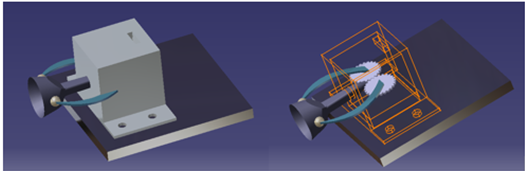
\includegraphics[scale=1.0]{figuras/ventosa.png}
		\caption{Conceito do mecanismo da ventosa}
		\label{ventosa}
\end{figure}

O conjunto completo responsável pela movimentação nos eixos “x” e “y” é apresentado na figura \ref{eixoy} e figura \ref{eixoy2}  em que é apresentado respectivamente a vista explodida do mecanismo e sua movimentação através das setas em vermelho.

\begin{figure}[H]
		\centering
			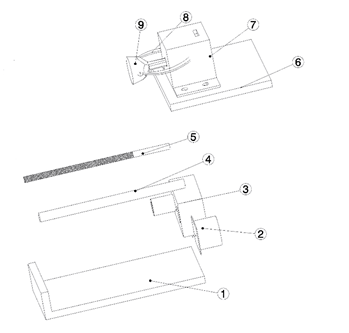
\includegraphics[scale=1.0]{figuras/eixoy.png}
		\caption{Mecanismo do eixo "y" em vista explodida}
		\label{eixoy}
\end{figure}

\begin{figure}[H]
		\centering
			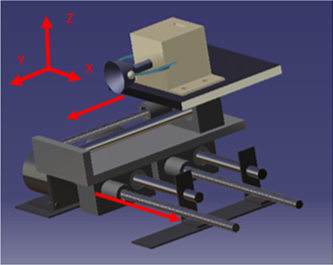
\includegraphics[scale=1.0]{figuras/eixoy2.png}
		\caption{Conceito do mecanismo completo de movimentação do eixo x e y}
		\label{eixoy2}
\end{figure}

A Figura \ref{eixoy3}, traz a lista dos principais componentes citados na na figura \ref{eixoy}. Em que assim como no mecanismo apresentado na seção anterior, os modelos são em sua maioria modelos comerciais, com exceção para o suporte de fixação da ventosa, a caixa de proteção dos sensores e a pinça.

\begin{figure}[H]
		\centering
			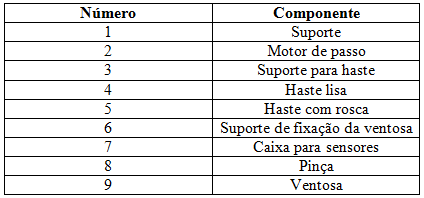
\includegraphics[scale=1.0]{figuras/eixoy3.png}
		\caption{Lista de componentes do eixo "y", referente a figura \ref{eixoy}}
		\label{eixoy3}
\end{figure}

\subsubsection[Mecanismo responsável pela movimentação em relação eixo z]{Mecanismo responsável pela movimentação em relação eixo z}

Para esta movimentação será utilizado um sistema mecânico que será calibrado por um profissional competente, o sistema de calibração será baseado nos percentis mais comuns do corpo humano, que serão obtidos utilizando o pacote de análise ergonômica disponível no software CATIA, que traz em sua biblioteca diversos manequins humanos. Desta forma, é possível estimar o tamanho médio dos prováveis usuários para atender com mais eficiência e agregar maior conforto ao equipamento.

O mecanismo responsável por este movimento será composto de um eixo móvel e um fixo desta forma será estabelecido segmentos em que o travamento deve ocorrer, através de um pino.



\subsection[Análise Ergonômica]{Análise Ergonômica}

Um dos objetivos do equipamento é ser uma máquina robusta, que pode ser adaptada para diversos tipos de usuários, para tanto foi necessário fazer um estudo de análise de conforto para diversos percentis de pessoas, fez-se uso da ferramenta RULA Analysis, dentro do ambiente de análise ergonômica do Software CATIA V5R19, esta ferramenta é capaz de fazer uma analise de conforto das principais partes do corpo humano a partir da sua posição.  

O primeiro perfil analisado foi de um usuário adulto entre 18-30 anos, com percentil 99,99\% cuja posição é sentado e imóvel, como vemos na figura \ref{adulto}.

\begin{figure}[H]
		\centering
			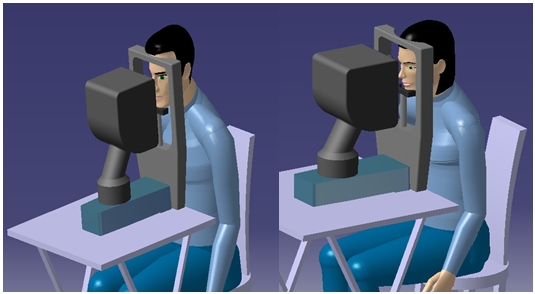
\includegraphics[scale=1.0]{figuras/adulto.png}
		\caption{Analise ergonômica para percentil 99\%}
		\label{adulto}
\end{figure}

Para este perfil de usuário as análises feitas pelo software foram satisfatórias, em uma escala de conforto que vai de 0 a 10, sendo 10 a posição mais desconfortável, a maior parte dos membros do usuário está em uma posição ergonomicamente confortável como mostra a figura \ref{adulto2}.

\begin{figure}[H]
		\centering
			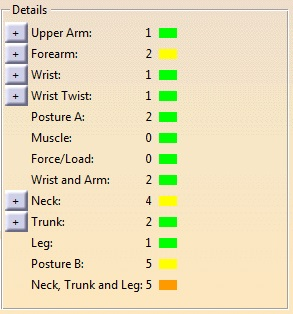
\includegraphics[scale=1.0]{figuras/adulto2.png}
		\caption{Resultado da análise de conforto}
		\label{adulto2}
\end{figure}

O segundo perfil estudado foi de um idoso a partir dos 60 anos, no qual sua posição também é sentada e considerada estática para colocação da lente de contato, como mostra a figura \ref{idoso}. 


\begin{figure}[H]
		\centering
			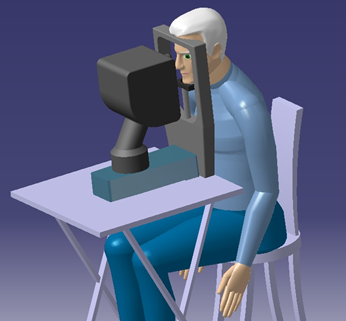
\includegraphics[scale=0.8]{figuras/idoso.png}
		\caption{Análise ergonômica para idoso}
		\label{idoso}
\end{figure}

Para o idoso alguns parâmetros mudaram, como o conforto do pescoço que ficou por volta de 7, no entanto este incomodo pode ser resolvido facilmente devido o local onde o queixo fica apoiado ser ajustável, assim a máquina atenderá a necessidade de colocar a lente de um idoso que possui dificuldades motoras.

Foi realizado também uma análise de conforto para o percentil de 50\%. Os resultados estão representados na figura \ref{idoso2}.


\begin{figure}[H]
		\centering
			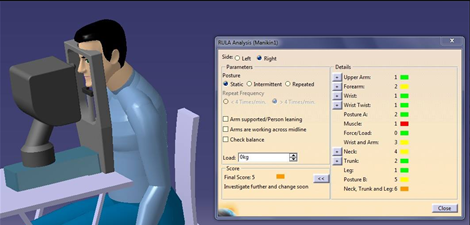
\includegraphics[scale=1.0]{figuras/idoso2.png}
		\caption{Resultado da análise de conforto para percentil de 50\%}
		\label{idoso2}
\end{figure}





\subsection[Sistema de Armazenamento]{Sistema de Armazenamento}

O sistema de armazenamento tem como principal objetivo armazenar as lentes de contato adequadamente e de forma funcional no aparelho.

O raio de curvatura médio da córnea humana é aproximadamente 7,8$mm$. O recipiente de armazenamento foi projeto para armazenar as lentes de contato de forma que o aplicador seja capaz de retirá-la do recipiente na posição correta para a aplicação no usuário.

Como as lentes de contato devem ficar imersas em um líquido hidratante, cujo pH é muito próximo ao pH da lágrima, o recipiente foi projetado para girar $90^\circ$, de tal forma que o líquido escorra para um lado do recipiente por simples ação da gravidade.

Ao acionar o sistema de rotação à $90^\circ$ do recipiente, o sistema de sucção acoplado ao recipiente será acionadas para que as lentes não saiam do lugar.

O recipiente de armazenamento está ilustrado na figura \ref{fig30}.

\begin{figure}[H]
		\centering
			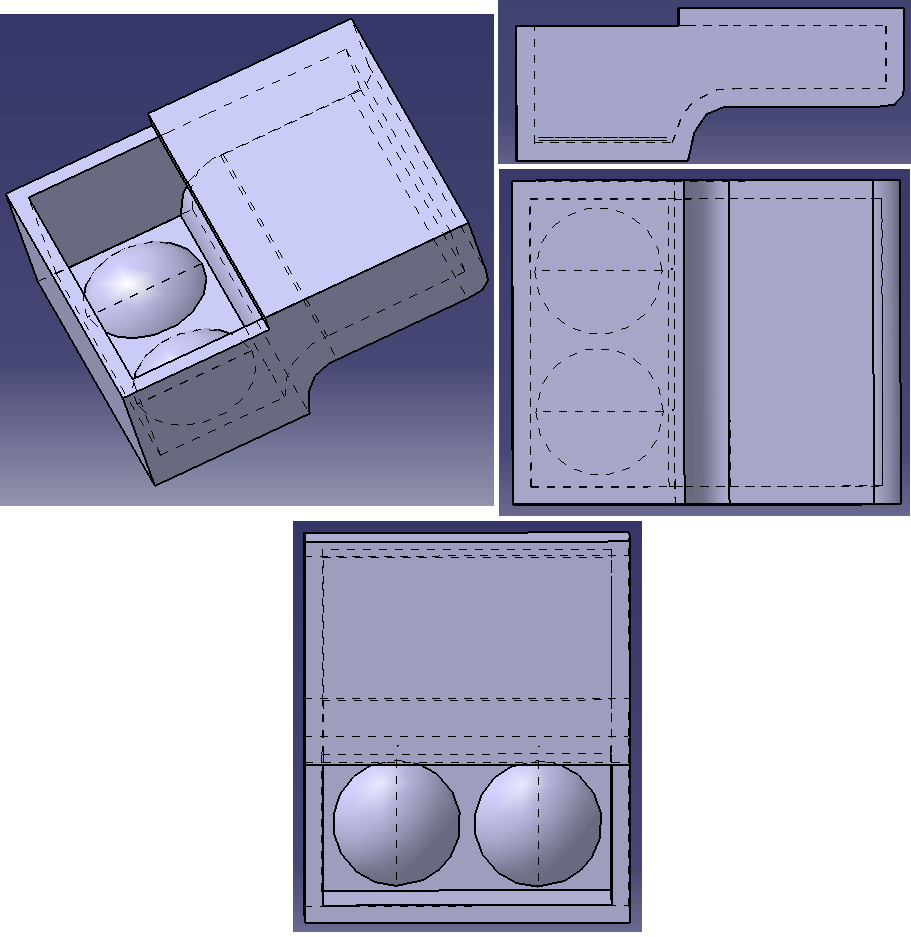
\includegraphics[scale= 0.6]{figuras/recipiente.png}
		\caption{Recipiente de Armazenamento}
		\label{fig30}
\end{figure}

As medidas da lente de contato utilizada nos testes e do recipiente estão expostas nas figuras \ref{caixamedidas} e \ref{lentemedidas}, respectivamente.


\begin{figure}[htb]
		\centering
			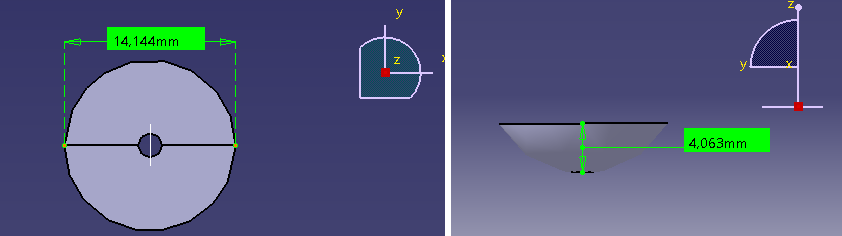
\includegraphics[scale=0.6]{figuras/lentemedidas.png}
		\caption{Cotas da lente de contato}
		\label{lentemedidas}
\end{figure}

\begin{figure}[htb]
		\centering
			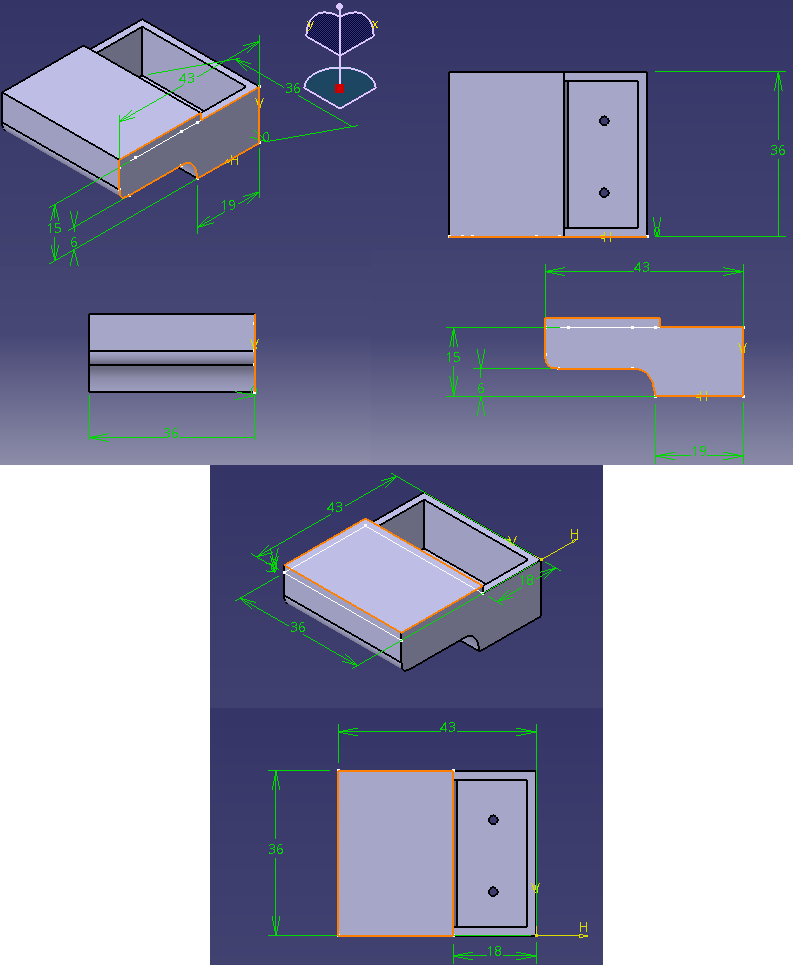
\includegraphics[scale=0.6]{figuras/caixamedidas.png}
		\caption{Cotas para o recipiente de armazenamento}
		\label{caixamedidas}
\end{figure}






\section[Sensores: justificativa de escolhas]{Sensores: justificativa de escolhas}

O objetivo maior da parte do projeto referente à instrumentação e sensoriamento é a detecção do toque da lente no globo ocular do usuário e evitar qualquer risco à saúde em meio ao procedimento de colocação e retirada das lentes de contato. Para atingir tal propósito, foi realizada uma vasta pesquisa sobre os sensores que poderiam responder bem aos requisitos de projeto. Foi pesquisado sobre sensores de toque, pressão, ultrassom e força, porém os que melhor atenderam ao propósito foram os de pressão e força. 

Após a delimitação do tipo de sensor, foram testados em laboratório sensores de força FlexiForce A201 e FSR 402 e 406, os quais alteram sua resistência em resposta à aplicação de força sobre sua área sensível, ativa. Esses sensores responderam muito bem aos estímulos feitos com a colocação de massas específicas em sua superfície ativa, porém o que  justificou a escolha do FRS 406 foi sua maior área ativa. Enquanto o FRS 402 apresenta área ativa de 12,7$mm$ de diâmetro o FRS 406 apresenta área ativa de 38,1$mm$ x 38,1$mm$ e o FlexiForce apresenta área ativa de 9,53$mm$ de diâmetro. Além disso, o tempo de resposta do FSR 406 é menor do que o do Flexiforce, 3 $\mu s$ e 5 $\mu s$, respectivamente.

Com relação aos sensores de pressão, foram testados os sensores MPXV5004DP e MPXM2010GS e o que justificou a escolha do MPXV5004DP foi a sensibilidade. Enquanto o MPXM2010GS apresenta sensibilidade de 2,5 $mV/KPa$, o MPXV5004DP apresenta sensibilidade de 1 $V/KPa$, ou seja, bem maior do que o anterior.

Destarte, haverá dois sensores para detectar o toque no olho: um principal, o FSR, que é mais confiável, e um sensor de redundância, o MPXV5004DP, para maximizar a segurança do usuário e como opção em caso do primeiro sensor falhar em meio ao procedimento. 

\subsection[Sensor de pressão MPXV5004DP]{Sensor de pressão MPXV5004DP}

O componente MPXV5004DP pertence à série de transdutores piezo-resistivos MPXX5004, que são sensores de pressão de silício monolítico concebidos para uma ampla gama de aplicações, mas particularmente as que usam um microcontrolador ou um microprocessador com entradas A/D. Esse sensor possui um medidor de deformação de alta sensibilidade, construído com avançadas técnicas de micro-usinagem, metalização de filme fino e processamento bipolar para fornecer um sinal de saída analógico com alto nível de acurácia, o qual é proporcional à pressão aplicada. Alguns exemplos da aplicação desse sensor são em equipamentos respiratórios, medições de pressão, verificação de nível de líquidos, sistemas baseados em microcontroladores ou microprocessadores.

Há três tipos de medida de pressão: pressão Gauge, pressão diferencial e pressão absoluta. A pressão Gauge é a diferença entre a pressão de interesse e a pressão ambiente. A pressão diferencial é a diferença de pressão entre dois pontos distintos em uma planta, onde estes dois pontos não estão necessariamente sob a pressão atmosférica. Já a pressão absoluta é medida por um sensor diferencial com um dos pontos em 0 psi, próximo ao vácuo total. O sensor MPXV5004DP se classifica como um medidor de pressão Gauge, onde mede-se a diferença entre a pressão extraocular e a pressão atmosférica, visando detectar o momento em que a ventosa toca o globo ocular.

O sensor MPXV5004DP mede pressões entre 0 e 400 $mmH_{2}O$, com tensões de saída entre 1,0 e 4,9V. A Figura \ref{sensor1} (a) ilustra o modelo comercial deste sensor, onde pode-se observar as duas entradas, uma para a pressão atmosférica e a outra para a pressão de interesse. A Figura \ref{sensor1} (b) ilustra a vista superior deste sensor, onde os pinos de 1 a 4 correspondem, respectivamente, ao GND, +VOUT, Vs, -VOUT; os outros pinos, de 5 a 8, não são utilizados.

\begin{figure}[htb]
		\centering
			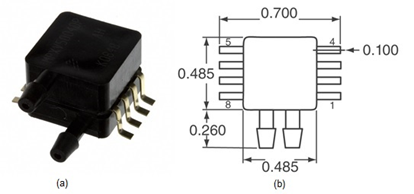
\includegraphics[scale=1.0]{figuras/sensor1.png}
		\caption{(a) Modelo comercial do sensor de pressão MPXV5004DP. (b) Datasheet do sensor MPXV5004DP e dimensões, onde os pinos de 1 a 4 correspondem, respectivamente, ao GND, +Vout, Vs, -Vout \cite{sensor1}}
		\label{sensor1}
\end{figure}

As características de operação do sensor MPXV5004DP com temperatura de operação 25ºC são apresentadas na figura \ref{caractsensor1}.

\begin{figure}[htb]
		\centering
			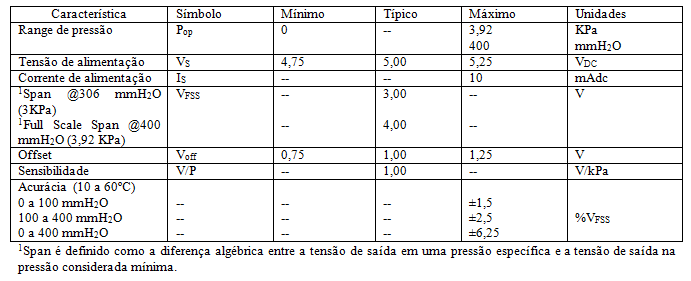
\includegraphics[scale=0.8]{figuras/caractsensor1.png}
		\caption{Características de operação do sensor MPXV5004DP \cite{sensor1} }
		\label{caractsensor1}
\end{figure}

\subsection[Sensor de força Flex Force 406]{Sensor de força Flex Force 406}

Force Sensing Resistors, ou FSR’s, são dispositivos robustos de filme espesso de polímero que exibem decréscimo na resistência com o aumento da força aplicada sobre a superfície do sensor, permitindo, assim, detecção de pressão física. A sensibilidade na detecção de força é otimizada para uso em controle de toque humano em dispositivos eletrônicos, sistemas médicos e em aplicações industriais e robóticas. Algumas das aplicações dos sensores FSR’s são para detectar e qualificar pressão, aumentar a segurança de instrumentos, detectar presença, posição e movimento, encontrar centro de força.

O FSR 406 tem forma quadrada com 43,69$mm$ de lado, com área ativa de 38,1$mm$ x 38,1$mm$. Como ilustrado na figura \ref{sensor2}.

\begin{figure}[htb]
		\centering
			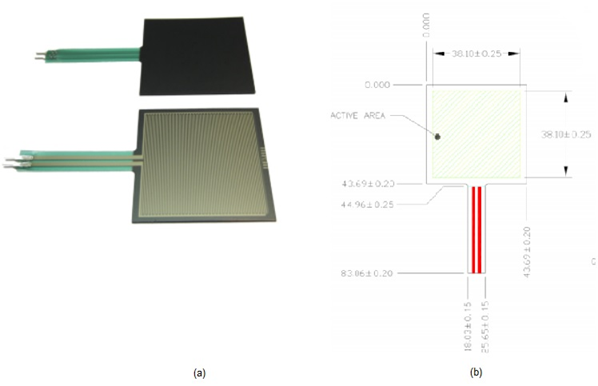
\includegraphics[scale=1.0]{figuras/sensor2.png}
		\caption{(a) Modelo comercial do sensor FSR 406. (B) Especificação das medidas do sensor FSR 406 \cite{sensor2}}
		\label{sensor2}
\end{figure}

As características do dispositivo FSR 406 são apresentadas na figura \ref{caractsensor2}. A tensão de alimentação utilizada durantes os procedimentos de teste foi de 5 V.

\begin{figure}[htb]
		\centering
			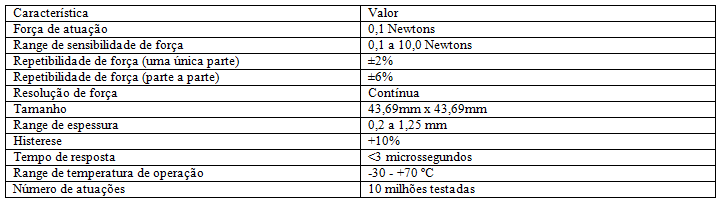
\includegraphics[scale=0.9]{figuras/caractsensor2.png}
		\caption{Características do sensor FSR 406 \cite{sensor2}}
		\label{caractsensor2}
\end{figure}

\subsection[Chave Óptica]{Chave Óptica}

Outro sensor a ser utilizado no aparelho é a chave óptica. Esse dispositivo apresenta uma tensão de saída de aproximadamente 20 mV quando a iluminação na chave é interrompida e de aproximadamente 5 mV quando a luz passa sem obstáculos através da chave. Este dispositivo tem o propósito de detectar quando a estrutura da ventosa e sensores chegou à posição do olho no eixo horizontal X. Haverá duas chaves, uma para cada olho, fixas e com igual propósito, ou seja, detectar quando a ventosa está posicionada em frente ao olho do usuário. Quando essa posição for atingida, o movimento em X cessará e será  iniciado o movimento em y, levando a lente em direção ao olho do usuário. Na estrutura que contém a pinça e a ventosa haverá um pequeno obturador posicionado estrategicamente de forma que ele interrompa a passagem de luz no sensor na posição em que se deseja colocar a lente. A Figura \ref{sensor3} ilustra tal dispositivo. O modelo a ser utilizado é o K733.

\begin{figure}[H]
		\centering
			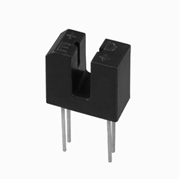
\includegraphics[scale=1.0]{figuras/sensor3.png}
		\caption{Modelo comercial da chave óptica}
		\label{sensor3}
\end{figure}


\section[Disposição dos sensores no equipamento]{Disposição dos sensores no equipamento}

Para que seja possível fazer o controle dos movimentos do produto é necessário que alguns sinais de controle sejam obtidos. Estes sinais em sua maioria serão advindos dos sensores mencionados anteriormente e espalhados pelo produto, exceto a detecção do olho está aberto ou não que será feito via processamento de imagens.
	
Desta forma, depois de definido os sensores que serão utilizados, conforme explicado acima, o próximo passo está em definir como os mesmos serão dispostos no produto e a maneira que será efetuado o circuito de interface que irá gerar as entradas de controle do código no Arduíno. Optou-se por utilizar neste produto um sensor de força FSR – Force Sensitive Resistor, um sensor de pressão de coluna de ar diferencial e duas chaves ópticas. 

O sensor de força FSR deverá ser fixado em uma superfície rígida, para que as medidas apresentadas por ele sejam confiáveis e apresentem repetitividade. Esta decisão foi motivada, ao verificar experimentalmente que o FSR só apresentava repetitividade nas medições quando se encontrava sobre uma superfície rígida. No caso do protótipo, optou-se por utilizar um pedaço de madeira onde o sensor foi colado, tomando os devidos cuidados para que o sensor esteja completamente aderido na superfície conforme mostrado na figura \ref{visaofl}. 

Em seguida foi colada uma borracha de dimensões 1,2x1,0x0,4 $cm$ no centro do FSR, sendo está borracha utilizada para que a área de contato do FSR seja sempre a mesma, reduzindo consideravelmente os erros na leitura do FSR que eram observados experimentalmente quando se alterava a área de contato, tornando desta forma a medição mais confiável (vide figura \ref{visaofl}). 

Logo em cima da borracha é colado o sensor de pressão de ar diferencial, sendo que a borracha foi cortada nas dimensões mencionada acima justamente devido a estas serem a dimensão do encapsulamento do sensor de pressão de ar. 

Assim, foi colocada uma ventosa para lente escleral com a parte posterior cortado em seção reta em uma das entradas do sensor de pressão. Após inserir a ventosa, tomaram-se os devidos cuidados para que a mesma fosse corretamente vedada de modo a evitar que ocorresse algum vazamento de ar que prejudicasse a medição do sensor de pressão. A outra entrada do sensor foi utilizada para pressão ambiente de referência do sensor.

\begin{figure}[H]
		\centering
			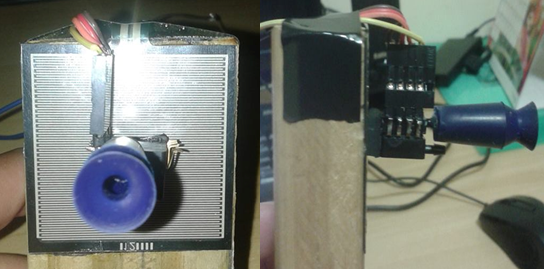
\includegraphics[scale=1.0]{figuras/visaofl.png}
		\caption{Vista frontal e lateral da disposição dos sensores}
		\label{visaofl}
\end{figure}

Com isso, tem-se a placa com o circuito de interface dos sensores, na parte posterior da madeira, sendo que os componentes escolhidos são em sua maioria SMD (do inglês \textit{Surface Mounted Device}), visando com isso obter uma área reduzida e reduzir a quantidade de cabos utilizados. O circuito de interface destes sensores será descrito melhor a seguir, onde será apresentado o esquemático do circuito. A confecção e teste da placa com o circuito de interface ainda não está concluído sendo um trabalho futuro neste projeto, porém o circuito já foi testado e validado em matriz de contato, estando também a parte de esquemático e roteamento da placa concluídos. Para a elaboração do esquemático e roteamento foi utilizado o software EAGLE 6.5.
	
Ainda haverá, nesta estrutura, uma pinça ao redor da ventosa que será utilizada para deformar a lente de modo que a mesma possa ser retirada com o contato da lente com a ventosa. Esta pinça ainda não está concluída, sendo também um dos trabalhos futuros deste produto figura \ref{caixa}.

Tem-se então a caixa que irá armazenar toda a estrutura acima que é uma caixa com dimensões 5,0x5,0x5,0 $cm$ que possui um orifício circular na parte frontal para saída da ventosa, um orifício retangular na parte superior para saída dos cabos de comunicação com os demais circuitos e dois orifícios laterais, um de cada lado, para a saída do mecanismo da pinça.

\begin{figure}[H]
		\centering
			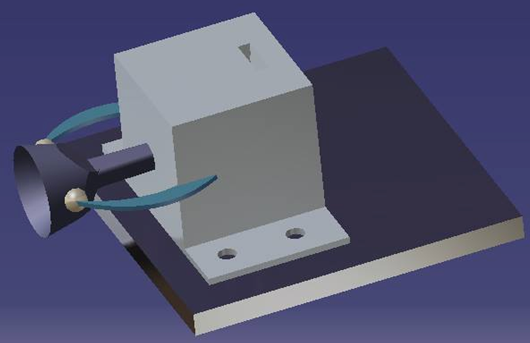
\includegraphics[scale=1.0]{figuras/caixa.png}
		\caption{Caixa de armazenamento dos sensores de pressão de ar diferencial, FSR e da placa que realiza a interface desses circuitos}
		\label{caixa}
\end{figure}

As chaves ópticas serão ajustadas para ficar exatamente na frente do olho do usuário, sendo uma chave óptica para cada olho, este ajuste da posição das chaves ópticas será efetuado através de uma calibração manual junto ao profissional competente. No caso destes sensores, eles ficarão fora da caixa, posicionados logo acima da mesma e ao longo do eixo X, presos em um estrutura adequada que permite seu ajuste.

Por fim, tem-se a placa de desenvolvimento do Arduino posicionada na parte posterior externa na caixa, sendo o mesmo utilizado para efetuar o algoritmo de controle e atuação do produto. Futuramente, pretende-se confeccionar uma placa que contenha apenas o microcontrolador e os componentes que serão utilizados para este produto de forma a minimizar a área ocupada e baratear o custo do projeto. A disposição física da placa de controle e das placas adicionais ainda será discutida e otimizada posteriormente.

\section[Circuito de interface dos sensores]{Circuito de interface dos sensores}

A interface, também conhecida como conformador de sinal ou pré-amplificador compatibiliza o sinal de saída do transdutor com as características de entrada exigidas pelos circuitos eletrônicos. No caso deste produto, a principal função dos circuitos de interface será obter sinais de controle digitais que entrarão nos pinos de I/O digitais do Arduino.
	
Conforme mencionado acima, o sensor FSR e o sensor de pressão diferencial estão na mesma placa, devido a maior parte dos sensores se encontrarem nesta placa, decidiu-se que esta será a placa responsável por fazer a comunicação com o Arduino e obter a alimentação oriunda do circuito controlador de carga do circuito.

Desta forma a placa que irá junto com o sensor FSR e de pressão diferencial, deverá conter um conector com dois pinos para entrada da tensão de alimentação conforme mostra afigura \ref{conectdiv}(b); dois reguladores de tensão, um que gera de saída uma tensão de 3,3V e outro que gera de saída uma tensão de 5V, onde os capacitores são apenas para desacoplamento (figura \ref{conectdiv}(a) e \ref{conectdiv}(c), respectivamente); dois conectores de três pinos que irão para as duas placas de interface da chave óptica, sendo os dois idênticos contendo a alimentação Vcc de 3,3V, terra e a saída digital do circuito de interface da chave óptica conforme figura \ref{conectdiv}(d) e figura \ref{conectdiv}(f); um conector de quatro pinos com as saídas digitais de todos os circuitos que irá para as entradas I/O digitais do Arduino é mostrado na figura \ref{conectdiv}(e). Por fim, os circuitos de interface dos sensores FSR e pressão diferencial serão explicados adequadamente a seguir.

\begin{figure}[H]
		\centering
			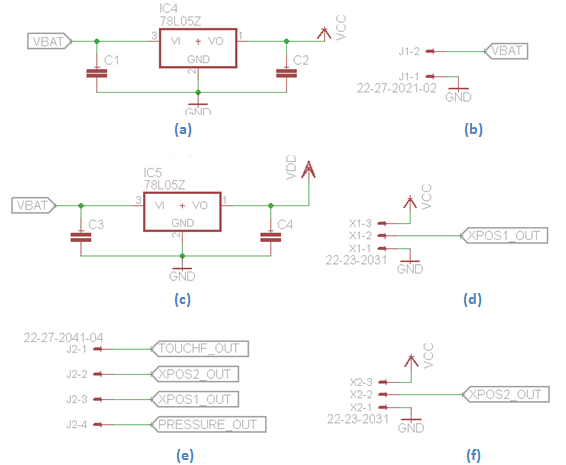
\includegraphics[scale=1.0]{figuras/conectdiv.png}
		\caption{Conectores e divisores de tensão da placa de interface dos sensores FSR e pressão de ar diferencial}
		\label{conectdiv}
\end{figure}

O sensor de pressão diferencial deve ser alimentado com 5V e terra e tem sua tensão de saída no pino 4 conforme expresso na figura \ref{circuito1}, basicamente quando detecta uma pressão na ponta da ventosa a tensão de saída que inicialmente fica por volta de 1,1V decai para um valor próximo de 0V. 

Desta forma uma boa maneira de obter uma saída digital do circuito é acoplando a saída do sensor a um comparador com tensão de referência de 0,9V. Assim, caso a tensão de saída seja maior que 0,9V, a saída do comparador será 0 e caso seja menor do que a tensão de referência, a saída do comparador será Vcc. Este amplificador será alimentado com 3,3V, que é a tensão de entrada para nível alto da porta I/O do Arduino. 

Vale ressaltar que ao tocar o olho a tensão de saída varia bruscamente, porém dependendo do movimento do usuário ela pode em alguns momentos voltar a tensão original de 1,1V, logo assim que detectar o primeiro nível alto já é necessário que o Arduino passe para o próximo estado. Para obter a tensão de referência é necessário fazer um divisor de tensão com dois resistores. Pela equação mostrada na figura \ref{circuito1}, considerando que desejamos uma tensão de 0,9V, a melhor escolha de resistores é $R_1 = 1,8 k\Omega$ e $R_2 = 8,2k\Omega$.

\begin{figure}[H]
		\centering
			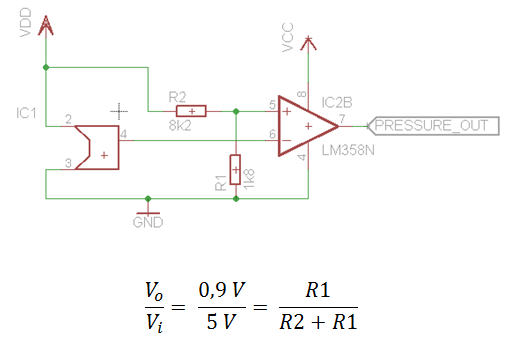
\includegraphics[scale=1.0]{figuras/circuito1.png}
		\caption{Circuito de interface do sensor de pressão de ar diferencial}
		\label{circuito1}
\end{figure}

Já o circuito de interface do FSR deve ser capaz de lidar com um sensor que diminui a resistência quando submetido ao toque, logo para tal a configuração adotada foi uma ponte de Wheatstone com amplificador operacional, de forma a minimizar a interferência do circuito a uma eventual carga (figura \ref{circuito2}). Neste circuito tem-se também um comparador de forma a tornar a saída do circuito em uma saída digital. 

\begin{figure}[H]
		\centering
			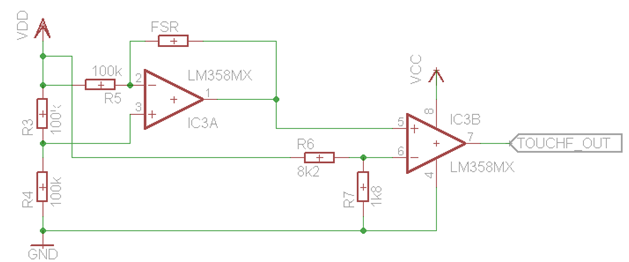
\includegraphics[scale=1.0]{figuras/circuito2.png}
		\caption{Circuito de interface do FSR}
		\label{circuito2}
\end{figure}

Em uma ponte de Wheatstone tem-se que os valores das resistências $R_3$, $R_4$ e $R_5$ são iguais a resistência do FSR sem carga; esta resistência é de aproximadamente 100 $k\Omega$. Desta forma, a tensão no pino 3 (entrada não inversora) do amplificador operacional é $VDD/2$ e, consequentemente, a tensão no pino 2 (entrada inversora) do amplificador operacional também é $VDD/2$. Isto faz com que a corrente que passa pelo FSR seja a mesma que passa pelo resistor $R_5$. Logo, a corrente que passa pelo sensor é dada pela equação mostrada na figura \ref{eq2}.

\begin{figure}[H]
		\centering
			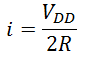
\includegraphics[scale=1.0]{figuras/eq2.png}
			\caption{Eq.2}
		\label{eq2}
\end{figure}

Dessa forma a tensão de saída pode ser descrita pela equação da figura \ref{eq3}, onde dr representa a variação de resistência no FSR e Vo é a tensão de saída da ponte de Wheatstone.

\begin{figure}[H]
		\centering
			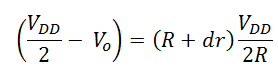
\includegraphics[scale=1.0]{figuras/eq3.png}
				\caption{Eq.3}
		\label{eq3}
\end{figure}

Reordenando os termos obtemos o resultado apresentado na equação da figura \ref{eq4}.

\begin{figure}[H]
		\centering
			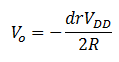
\includegraphics[scale=1.0]{figuras/eq4.png}
				\caption{Eq.4}
		\label{eq4}
\end{figure}

Resultado este que faz todo o sentido, já que ao pressionar o FSR obtemos uma queda brusca na resistência de forma que a variação dr é negativa e produz um aumento significativo na tensão de saída, que por sua vez estará limitada a $VDD/2$. Experimentalmente, a saída da ponte de Wheatstone, quando ocorria o toque no olho, era acima de 1V, e sem o toque este valor era de aproximadamente 0V. Desta forma, tomamos novamente 0,9V de tensão de referência, de forma a poder adotar os mesmos valores de resistores para $R_6$ e $R_7$ do circuito comparador anterior. Logo quando for detectado o toque no olho a saída TOUCH\_OUT será 1 e caso o contrário será 0.

Conforme mencionado, os circuitos de interface apresentados anteriormente estão localizados na mesma placa, porém através dos conectores percebemos que elas se comunicam com o Arduino, com o circuito de carga do produto e com ambas as placas da chave óptica. Logo, é importante também citar como é o circuito de interface das chaves ópticas, já que este também gera sinais de controle advindos de sensoriamento que será uma entrada do Arduino.

Sendo assim, cabe ressaltar que o sensor que será utilizado gera uma pequena variação na tensão quando algum objeto interrompe a luz, e, portanto é necessário que este sinal seja amplificado para que possa ser tratado mais facilmente, desta forma a interface deste circuito é realizado através do circuito apresentado na figura \ref{circuito3}.

A chave óptica fornece uma tensão de aproximadamente 20$mV$ quando a luz é interrompida e de 5$mV$ sem interrupção. Como o sinal é bem pequeno, ele precisa ser amplificado. Para isto, como mostrado na figura \ref{circuito3}, foi utilizado $R_1$, $R_2$, $R_3$ com o valor de 1$k\Omega$ e o resistor $R_4$ com 100$k\Omega$. Isto acaba ocasionando um ganho alto ao sistema e como a frequência que o sistema precisa operar é bem baixa, este ganho acaba não causando problemas para o funcionamento do circuito. Por fim, tem-se um comparador capaz de tornar digital a saída da chave óptica, onde a saída é 1 quando a posição em X está interrompendo o sensor e 0 caso contrário.

\begin{figure}[H]
		\centering
			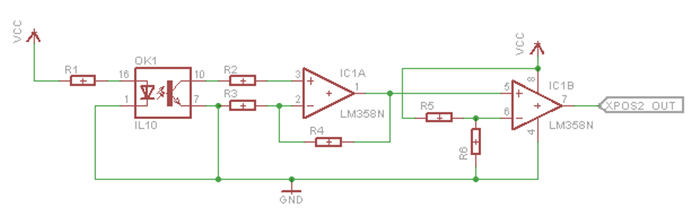
\includegraphics[scale=0.9]{figuras/circuito3.png}
		\caption{Circuito de interface da chave óptica}
		\label{circuito3}
\end{figure}

Neste circuito temos também três conectores que estarão ligados na placa dos sensores de força e pressão de ar diferencial. Destes conectores será provida alimentação do circuito de 3,3 V, o GND do circuito e será enviado para a placa de interface dos sensores de força e de pressão a saída digital da posição em X figura \ref{conectchave}.

\begin{figure}[H]
		\centering
			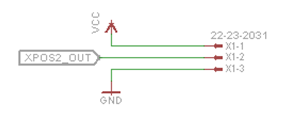
\includegraphics[scale=1.0]{figuras/conectchave.png}
		\caption{Conector presente na placa da chave óptica}
		\label{conectchave}
\end{figure}

Vale lembrar que as duas placas de interface da chave óptica possuem o mesmo circuito, alterando apenas a nome da saída.

\section[Processamento de Imagens - O Safety do Posicionador de Lente]{Processamento de Imagens - O Safety do Posicionador de Lente}

Para assegurar que o usuário do Posicionador de Lente está posicionado no lugar correto e está com o olho aberto de forma adequada para a inserção ou retirada da lente foi desenvolvido um algoritmo de processamento de imagem, o qual detecta se o olho do usuário está aberto e interrompe o funcionamento do produto caso o mesmo esteja fechado ou fora da posição adequada.

A construção do algoritmo de detecção do olho aberto ou fechado foi segmentada em quatro etapas. Detecção da face, detecção do olho, detecção da íris e classificação do estado do olho em aberto ou fechado para assim determinar se o equipamento pode avançar ou não. Para o algoritmo implementado considerou-se que o rosto do usuário encontra-se fixo e imóvel a uma distância média da câmera de pelo menos 20cm e que as condições de iluminação estão adequadas.

Foi utilizada a linguagem Python juntamente com a biblioteca OpenCV, que foi desenvolvida essencialmente para aplicações de processamento de imagens e possui muitas ferramentas que facilitam esse tipo de aplicação. 

A implementação aqui descrita foi baseada no algoritmo proposto por \citeonline{viola}, onde se usa elementos de detecção previamente treinados (Haar-like features) para a classificação. Estes elementos estão disponíveis nas bibliotecas utilizadas em processamento de imagens como a OpenCV. 

Na detecção do rosto foi utilizado o classificador da face frontal (haarcascade \_frontalface\_default.xml). A partir deste, o código identifica os candidatos mais prováveis a face. Sabendo que a câmera está perto do rosto o algoritmo escolhe somente a maior região dentre as detectadas como prováveis rostos. Em seguida desenha um retângulo em volta da região para facilitar a visualização do resultado. 

Para encontrar as possíveis regiões para a presença do olho foi utilizado novamente o algoritmo de Viola-Jone (2001). Porém utilizando o classificador de olhos (haarcascade\_eye.xml). O detector foi então aplicado na região da face. Com isso foi possível encontrar as regiões mais prováveis para o olho. Em seguida desenhou-se um retângulo em volta da região para facilitar a visualização do resultado.  A imagem obtida pode ser vista na \ref{faceolho}.

\begin{figure}[H]
		\centering
			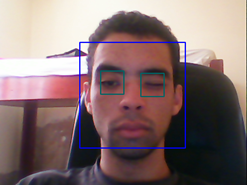
\includegraphics[scale=1.0]{figuras/faceolho.png}
		\caption{Detecção da face e do olho}
		\label{faceolho}
\end{figure}

Com o objetivo de saber se o equipamento deve ou não avançar é importante saber se o a íris está totalmente exposta. Uma ótima forma de encontrar objetos circulares em processamento de imagens é a transfomada de Rough, como é descrito por \citeonline{duarte}. Portanto ela foi utilizada para detectar a íris dentro da região previamente detectada como olho. 

Para que esta transformada detecte com precisão a região da íris é necessário que o olho esteja bem aberto. Condição que será atendida já que o olho do usuário será mantido aberto por uma pinça. O resultado de sua implementação pode ser visto na figura \ref{rough}, na qual foi necessário segurar a pálpebra inferior para expor a íris completamente.


\begin{figure}[H]
		\centering
			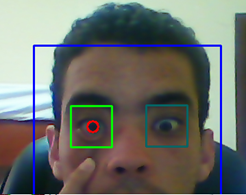
\includegraphics[scale=1.0]{figuras/rough.png}
		\caption{Detecção da íris através da transformada de Rough}
		\label{rough}
\end{figure}

É importante observar que as imagens aqui apresentadas são somente para ilustrar o processo e os resultados obtidos, pois, no produto final, o hardware desenvolvido a partir de um Raspberry Pi apenas fornecerá o estado atual do olho do usuário para o equipamento. O código desenvolvido pode ser encontrado no Apêndice C, D e E.



\section[Implementação da Lógica de Controle]{Implementação da Lógica de Controle}

A lógica de controle representa a sequências de movimentos que devem ser realizados para que o dispositivo cumpra a sua função. Em um nível de abstração mais alto, esta lógica pode ser representada por fluxograma que apresenta a ordem dos movimentos executados em função das entradas que são: sinal de comando do usuário e sinal de sensores. Em termos de implementação a lógica de controle é representada ou por um esquemático elétrico do hardware de controle ou pelo código do firmware de controle que apresenta como cada sinal de entrada é lido e quais os sinais de controle enviados para cada atuador, além da relação entre entrada, saída e tempo. Neste trabalho, optou-se por implementar a lógica de controle em Firmware embarcado em Arduino Mega 2560. O Arduino foi escolhido pela quantidade de GPIOs e saídas PWM disponíveis. Neste tópico será apresentada o desenvolvimento do firmware cujo o código está disponível em Apêndices. 

O procedimento de inserção e remoção da lente foi dividido em tarefas, em que cada tarefa só começa após o fim da tarefa anterior e próxima tarefa a ser executada depende da tarefa atual e das entradas. O código foi implementado baseado no modelo de máquinas de estados finitos em que cada estado representa uma tarefa e a transição entre os estados depende do estado atual e das entradas, e a saída de cada estado são os sinais de controle enviados para os atuadores.  A seguir serão apresentados os estados e suas implementações, mas primeiro vamos apresentar as entradas e saídas.

Todas as entradas são tratadas como entradas digitais, e são elas:
\begin{enumerate}
\item Comando de usuário para remover a lente.
\item Comando de usuário para inserir a lente.
\item Posição X 1:  Sinal enviado pela chave óptica que indica se o conjunto de atuadores está ou na frente do olho 1;
\item Posição X 2: Sinal enviado pela chave óptica que indica se o conjunto de atuadores está ou na frente do olho 2;
\item Toque por pressão: Sinal enviado pelo sensor de pressão do ar na ventosa que indica se o a ventosa está ou não em contato com olho. 
\item Toque por força: Sinal enviado pelo sensor resistivo FSR – Force Sensitive Resistor que indica se a ventosa está ou não em contato com o olho. 
\item Sinal enviado pelo algoritmo de processamento de imagem que indica se o olho está ou não aberto.
\end{enumerate}

As saídas do algoritmo são:
\begin{enumerate}
\item Sinal de comando dos dois motores de passo sincronizados de atuação no eixo X. 
\item Sinal de comando do motor de passo de atuação no eixo Y
\item Sinal de comando do servo motor de atuação na pinça de abertura do olho. 
\item Sinal de comando do servo motor de atuação na pinça de remoção da lente
\item Sinal de comando do servo motor de giro da caixa de armazenamento da lente. 
\end{enumerate}


\subsection{Estados}

\textbf{A)	STANDBY}

O estado STANDBY é o estado inicial, neste estado o sistema aguarda que o usuário insira um comando de retirar ou colocar a lente de contato, enquanto nenhum comando é inserido o Arduino permanece em modo de baixo consumo. 

O modo de baixo de consumo é obtido configurando o Arduino para SleepMode, o Arduino permanecerá neste estado até que uma interrupção ocorra. Um comando é reconhecido por uma borda de subida em um dos pinos em que estão conectados os botões de comando do usuário. Os botões são conectados em pinos capazes de disparar interrupções por I/O (pin. 2 e pin. 3) para que o Arduino seja retirado do SleepMode quando o usuário apertar um dos botões.

Neste estado todos os atuadores são mantidos parados.


\textbf{B)	PEGAR OU GUARDAR A LENTE NA CAIXA}

Este estado representa a tarefa de pegar ou guardar uma das lentes na caixa de armazenamento, em relação ao movimentos necessários, essas duas tarefas são iguais, a única diferença é a validação final que deve verificar se a lente foi aderida ou solta. Além dos sinais de entrada, este estado depende de uma variável interna conta olhos que indica qual das lentes deve ser pega. Esta tarefa é dividida nas ações de colocar a caixa de armazenamento de lentes na vertical, movimentar a ventosa no eixo X até que ela fique na frente da lente, mover a ventosa no eixo Y até ocorrer o contato ventosa-lente-caixa, e recuar a ventosa para a posição Y inicial.

O movimento da caixa de lentes é feito por um servo motor, então para essa sub tarefa basta comandar que o servo fique na angulação desejada. Esta angulação será determinada experimentalmente com os critérios de que a lente não escorregue, que o ângulo seja suficiente para escorrer suficientemente o líquido presente na caixa para conservar a lente de modo que a ventosa consiga retirar ou depositar a lente na caixa. O comando de posicionamento do servo não depende da posição inicial, assim não é necessário identificar inicialmente a orientação da caixa. 

A posição X das lentes de contato na caixa é fixa e representada no código pela quantidade de passos dos motores de atuação no eixo X entre a posição inicial e a posição da lente. Para colocar a ventosa na posição de armazenamento da lente de contato comanda-se que os motores de atuação X movam uma quantidade de passos igual a passos-POSLENTE\_I em que passos é uma variável que armazena a posição atual em passos da ventosa e POSLENTE\_I é uma constante que indica a posição em passos da lente i, o índice i indica qual das duas lentes. Se o resultado for positivo o movimento será para direita caso contrário será para esquerda.  Ao final do movimento a variável passosx deve ser atualizada para o valor da constante POSLENTE\_I.

A distância em Y entre a posição inicial da ventosa e as lentes é fixa e representada no código pela constante POSLENTEY que indica a quantidade de passos que motor de atuação no eixo Y precisa dar para levar a ventosa até a caixa.   Para mover a ventosa até a caixa basta comandar que o motor de passo mova uma quantidade passos igual a POSLENT, para recuar a ventosa basta comandar que motor de passo mova uma quantidade de passos igual a menos POSLENT. 

Antes de enviar o comando de recuo da ventosa é preciso verificar se a lente foi aderida pela ventosa, caso o comando de usuário seja COLOCAR, ou verificar se a lente foi depositada na caixa, caso o comando de usuário seja RETIRAR. Essa verificação é feita pelo sinal de Toque por pressão que é gerado pelo sensor que mede a pressão da coluna de ar na ventosa. Um problema a ser resolvido futuramente é o mecanismo usado para que a lente seja transferida da ventosa para a caixa.
 

\textbf{C)	MOVER PARA DIREITA}

Este estado representa a tarefa de movimentar a ventosa para direita até que ela fique na frente de um dos olhos. Além dos sinais de entrada, este estado depende da variável interna contaolhos que indica para qual dos olhos a ventosa deve ir. 

O posição de cada olho é marcado por um sensor de fim de curso que geram os sinais de entrada Posição X1 e Posição X2. O movimento para direita é implementado em um laço que repete continuamente os comandos a seguir até que o sinal Posição Xi indique a ventosa chegou na frente do olho.  

\begin{enumerate}
\item Move um passo 
\item Incrementa variável passos
\item Lê entrada Posição X1 ou Posição X2. 
\item Se for 1 a Posição Xi de interesse cessa o movimento, se for 0 volta para o comando 1.
\end{enumerate}


\textbf{D)	ABRIR O OLHO}

Este estado representa a tarefa de abrir o olho do usuário com uma pinça que o manterá aberta. O procedimento de abertura consiste em colocar a pinça em uma abertura inicial, esperar alguns poucos segundos para acomodação do usuário e em seguida colocar a pinça em uma abertura final maior do que a inicial. A abertura da pinça é controlada por um servo motor, então para controle da abertura da lente basta comandar que o servo fique em uma angulação desejada. Esta angulação será determinada experimentalmente. 

Por motivo de segurança e para obter a garantia de que a pinça conseguiu abrir os olhos do usuário, será monitorado através de processamento de imagens se o olho do usuário está ou não aberto. Caso não esteja aberto o movimento de mover para frente não pode ser realizado e a pinça volta a angulação inicial para uma nova acomodação do usuário. 


\textbf{E)	MOVER PARA FRENTE}

Este estado representa a tarefa de mover a ventosa até o olho, seja para inserir ou remover a lente. Esta tarefa é implementada em um laço que repete continuamente os comandos a seguir até que os sinais de toque por pressão ou toque por força indique que a ventosa tocou o olho ou a entrada Olho Aberto indique que o olho está fechado. 

\begin{enumerate}
\item Move um passo.
\item Incrementa variável passosy.
\item Lê entradas Toque por pressão, Toque por força e Olho Aberto. 
\item Volta a comando 1 enquanto não for detectado toque por força ou toque por pressão ou olho fechado.
\end{enumerate}

\textbf{F)	TIRAR A LENTE}

Este estado representa a tarefa de mover a pinça que causa uma deformação na lente para que ela possa ser retirada. A pinça de remoção é controlada por servo motor, então para execução desta tarefa basta comandar que o servo fique na orientação desejada. Está orientação será definida experimentalmente.

Este estado será executado logo após o estado E, somente quando estiver com sinal de remoção de lente em alto. 


\textbf{G)	MOVER PARA TRÁS}

Este estado representa a tarefa de mover a ventosa no eixo Y na direção contrária ao olho. A variável passosy armazena a quantidade de passos devem ser recuados até que a ventosa fique na posição inicial. Além de recuar a ventosa é necessário neste estado voltar a pinça de remoção da lente para posição inicial. A implementação desta tarefa consiste enviar o comando para o motor de atuação no eixo Y recue passosy, em seguida enviar o comando para que o servo motor de controle da pinça de remoção da lente fique na orientação inicial, e por último a variável passosy deve ser zerada. 

 
\textbf{H) RETORNAR À POSIÇÃO INICIAL}

Este estado representa o final do processo de inserção ou remoção da lente em que a ventosa deve voltar para a posição inicial. A posição atual da ventosa em quantidade de passos que o par de atuadores no eixo X precisam mover da posição inicial até a posição atual pode ser consultada na variável passosx, assim para mover até a posição inicial basta enviar o comando para que o par de atuadores andem –passosx¸ na conversão adotada o sinal negativo indica que os passos são em direção a posição inicial. 


\section[Acionamento dos Motores]{Acionamento dos Motores}
	
No caso deste projeto, foram utilizados três motores de passo do tipo unipolar. Esta escolha foi feita pelo fato do controle deste tipo de motor ser mais simples e o projeto da placa ser mais reduzido e barato. As fundamentações teóricas do funcionamento dos motores de passo encontram-se em anexo e podem ser consultadas para sanar eventuais dúvidas. Dois dos motores são para fazer o deslocamento no eixo X do aplicador de lente. A figura \ref{tabmotor1} mostra as especificações nominais do motor e a figura \ref{motor1} mostra a imagem do motor.

\begin{figure}[H]
		\centering
			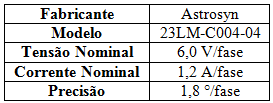
\includegraphics[scale=1.0]{figuras/tabmotor1.png}
		\caption{Características nominais do motor de passo Astrosyn}
		\label{tabmotor1}
\end{figure}

\begin{figure}[H]
		\centering
			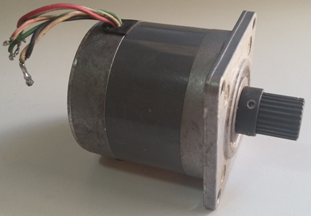
\includegraphics[scale=1.0]{figuras/motor1.png}
		\caption{Motor de Passo Astrosyn 23LM-C004-04}
		\label{motor1}
\end{figure}

O outro motor é utilizado para possibilitar o avanço em Y para o aplicador de lentes. A figura \ref{tabmotor2} mostra suas especificações nominais e a figura \ref{motor2} mostra a imagem do motor.

\begin{figure}[H]
		\centering
			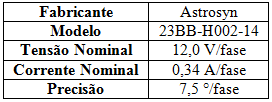
\includegraphics[scale=1.0]{figuras/tabmotor2.png}
		\caption{Características nominais do motor de passo Astrosyn}
		\label{tabmotor2}
\end{figure}

\begin{figure}[H]
		\centering
			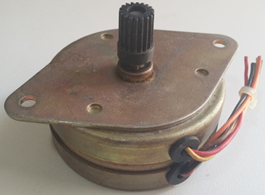
\includegraphics[scale=1.0]{figuras/motor2.png}
		\caption{Motor de Passo Astrosyn 23LM-C004-04}
		\label{motor2}
\end{figure}

Os três servomotores utilizados neste projeto são para levantar o compartimento das lentes (estojo) no momento da captura da lente, para abrir e fechar a pinça que mantém os olhos do usuário aberto e para pressionar a ventosa no momento da retirada da lente. Os servomotores não necessitam de placa para condicionamento de sinal e adequação dos níveis de tensão, pois são controlados através de sinal PWM vindo direto do microcontrolador e são alimentados com 5V, tensão que pode ser obtida diretamente da placa do Arduino. O modelo de servomotor utilizado é o SG90 da marca TowerPro (figura \ref{sg90}). Este servomotor é utilizado em aeromodelismo, mas devido às suas características, tem sido vastamente utilizado em aplicações de robótica. Suas características são:
\begin{itemize}
	\item Torque: 1,5 kg.cm
	\item Velocidade de operação: 0,1 s/60 graus
	\item Tensão de operação: 5V
	\item Peso: 9g
	\item Corrente de consumo: máximo de 0,4A 
\end{itemize}

\begin{figure}[H]
		\centering
			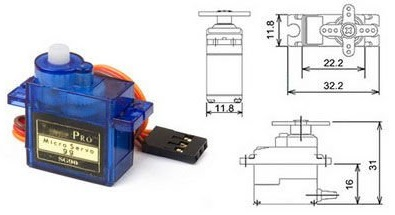
\includegraphics[scale=1.0]{figuras/SG90.png}
		\caption{Servomotor TowerPro SG90}
		\label{sg90}
\end{figure}


\section[Placa de Acionamento para Motores de Passo]{Placa de Acionamento para Motores de Passo}

Foi desenvolvida uma placa de acionamento dos motores de passo somente com componentes discretos. Apesar de ser possível encontrar no mercado circuitos integrados voltados para o acionamento de motores de passo, a capacidade de corrente fornecida por estes circuitos é limitada, logo houve a necessidade de se montar um circuito dedicado que oferecesse maior capacidade de corrente para os motores em uso.

Basicamente o circuito amplifica a tensão e/ou a corrente para o motor através de transistores bipolares tipo NPN como mostrado na figura \ref{esquematico2}. Existe um transistor para cada enrolamento e a entrada de alimentação deve ser proveniente de uma fonte de energia com tensão e correntes que suportem o funcionamento do motor. Os sinais de acionamento servem somente para comutar os transistores entre o corte e a saturação e são advindos do microcontrolador.

\begin{figure}[htb]
		\centering
			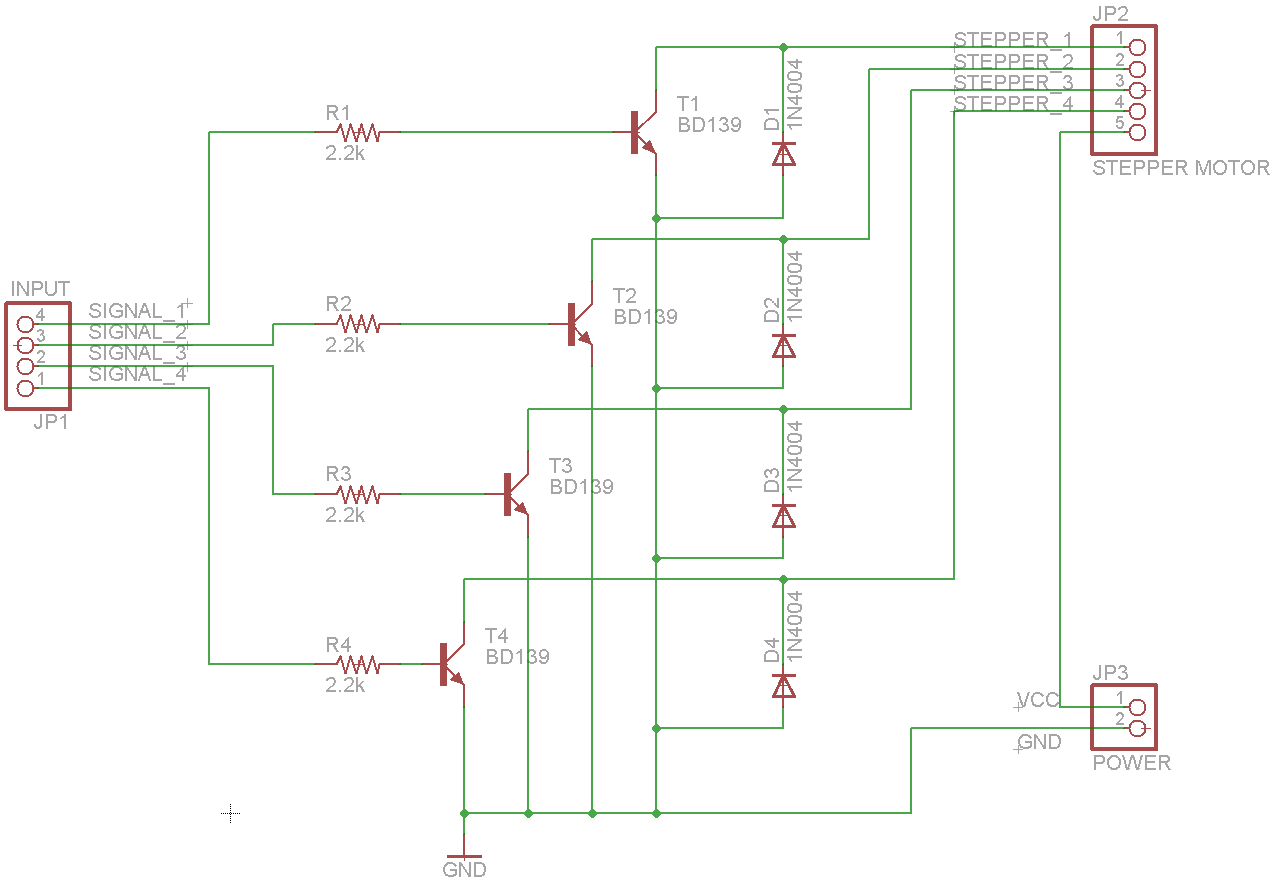
\includegraphics[scale=0.5]{figuras/esquematico2.png}
		\caption{Esquemático do circuito de acionamento dos motores de passo}
		\label{esquematico2}
\end{figure}

Os diodos 1N4004 ficam em paralelo com cada enrolamento do motor para que, quando o respectivo transistor entrar em corte, a energia (tensão reversa) produzida pelo campo magnético no enrolamento seja dissipada.

Os transistores BD139 suportam uma tensão coletor-emissor de até 80V e uma corrente de coletor de até 1,5A. Isto garante que eles irão trabalhar com uma boa folga, sabendo que a maior corrente que pode ser drenada pelos motores é de 1,2A. Os resistores ($R_1$, $R_2$, $R_3$ e $R_4$,) são todos de filme de carbono com potência de 1/8W. Os diodos 1N4004 suportam uma tensão reversa de até 400V e também trabalharão com folga aceitável, garantindo vida útil longa aos componentes.

Aplicando a Lei de Kirchhoff à malha base-emissor, obtém-se:

\begin{figure}[H]
		\centering
			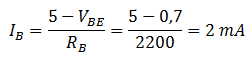
\includegraphics[scale=1.0]{figuras/leidek.png}
		\caption{Aplicação  a Lei de Kirchhoff à malha base-emissor}
		\label{leidek}
\end{figure}

Esta corrente irá garantir que o transistor entre na região de saturação para permitir o acionamento de cada enrolamento.

Na figura \ref{layout} é mostrado o layout da placa para o circuito proposto e a disposição dos componentes.

\begin{figure}[H]
		\centering
			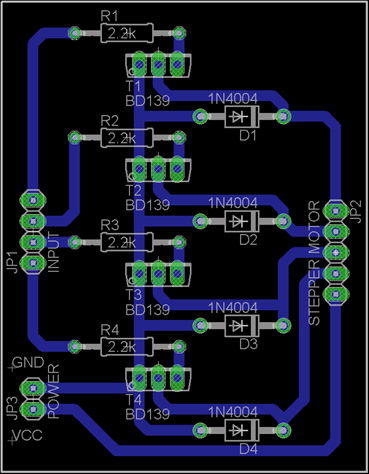
\includegraphics[scale=1.0]{figuras/layout.png}
		\caption{Layout do circuito de acionamento dos motores de passo}
		\label{layout}
\end{figure}


\section[Simulação da Modelagem Matemática]{Simulação da Modelagem Matemática}

Pensando na escolha dos motores para o projeto, foi desenvolvido um software de comparação e teste para motores DC  no MATLAB.

Para verificar o funcionamento do Servo Motor, foi analisada a função de transferência com a resposta impulsional e degrau. Onde mostra a relação de entrada e saída, que neste caso é a tensão pela posição analisadas ao longo do tempo.

Os parâmetros como Inércia, Indutância e resistência podem ser escolhidos pelo usuário do sistema, usando para isto a ferramenta GUI do Matlab. Com isto, diversos motores DC podem ser comparados de acordo com seus parâmetros, verificando a resposta dos motores que o Grupo possui, mostrando como o controle de posição e servindo de análise para aquisição de novos motores.

Na Figura \ref{simulacao1}, é mostrada a interface do usuário na resposta dos motores.

\begin{figure}[H]
		\centering
			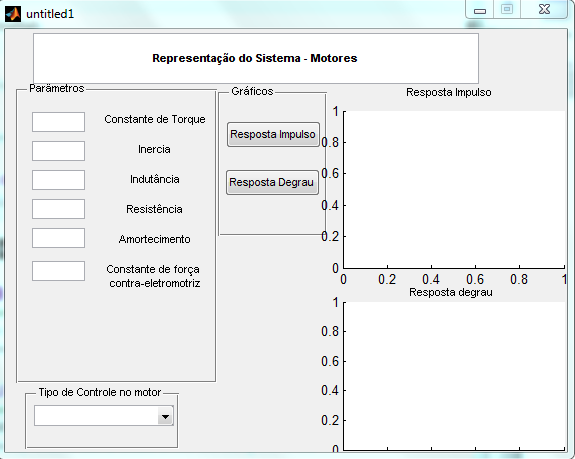
\includegraphics[scale=1.0]{figuras/simulacao1.png}
		\caption{Interface do usuário com a ferramenta GUI do Matlab}
		\label{simulacao1}
\end{figure}

Nesta Interface, é possível realizar a escolha dos parâmetros e do tipo de controle do motor (por armadura ou corrente de campo).

\textbf{Controle pela tensão aplicada na armadura}
No controle pela armadura mantém-se a tensão e a corrente no campo constante, desta forma o fluxo magnético produzido pelo campo também é constante. Varia-se a tensão aplicada na armadura (V) e por consequência a rotação da máquina, seguindo uma relação direta entre a tensão da armadura e a rotação da máquina. Neste método o torque permanece constante e a potência varia proporcionalmente com a velocidade.

\textbf{Controle pela tensão aplicada no campo}
No controle pelo campo, mantém-se a tensão de armadura constante e varia-se a corrente de excitação (Ia). Como o fluxo magnético é proporcional a corrente de excitação, diminuindo-se Ia, diminui-se o fluxo magnético "phi" e aumenta-se a velocidade de rotação n da máquina. No controle de campo a potência permanece constante enquanto a rotação se eleva e o torque se reduz. Este processo de aumento da velocidade de rotação pela diminuição do fluxo é conhecido por enfraquecimento de campo.

Com estas incógnitas inseridas pelo usuário, são dados os gráficos de resposta da saída, mostrado na figura \ref{simulacao2}.

\begin{figure}[H]
		\centering
			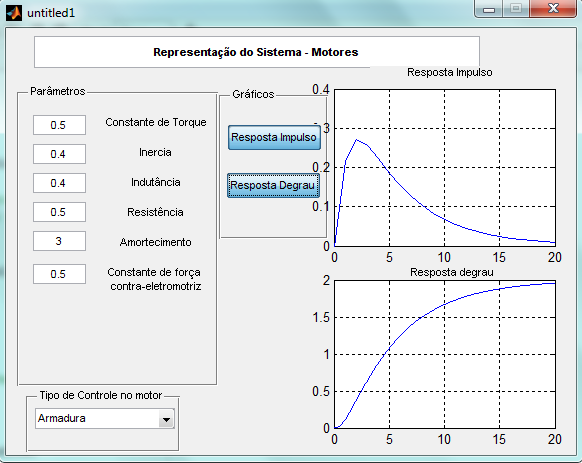
\includegraphics[scale=1.0]{figuras/simulacao2.png}
		\caption{Interface com as incógnitas especificadas}
		\label{simulacao2}
\end{figure}

As grandezas utilizadas nos parâmetros do motor estão no SI e o tempo está em milissegundos. No exemplo acima, a relação tensão e posição do motor, tem seu valor máximo entre 0 e 5 milissegundos.

\section[Bomba Peristáltica]{Bomba Peristáltica}

A bomba peristáltica é assim denominada em razão de seu movimento, que é muito similar ao peristaltismo do sistema digestório humano, que consiste em deslocar o alimento no tubo digestivo através de movimentos consecutivos de contração e relaxamento.

Conforme explicitado no manual da Bomba Peristáltica Vallair – Stenner, a bomba peristáltica consiste em um rotor com roletes dispostos em volta, os quais pressionam um tubo maleável e fixo, fechando-o e, portanto, criando o vácuo necessário para o deslocamento do fluido. Após a passagem do mesmo pelo rolete, o tubo retorna ao formato original, devido à memória mecânica de seu material de fabricação. O fluido não é submetido à contaminação, tendo em vista que, durante seu trajeto, este não entra em contato com nenhuma parte da bomba que não seja o tubo. Considerando que o fluido em questão será o responsável pela limpeza da lente, é de extrema importância que ele não seja danificado de forma alguma, e a bomba peristáltica atende a este pré-requisito, o que é uma das vantagens de utilizá-la no presente projeto.

A bomba peristáltica utilizada foi baseado em uma das partes de uma arma de brinquedo e está retratada na figura \ref{bomba}.

\begin{figure}[H]
		\centering
			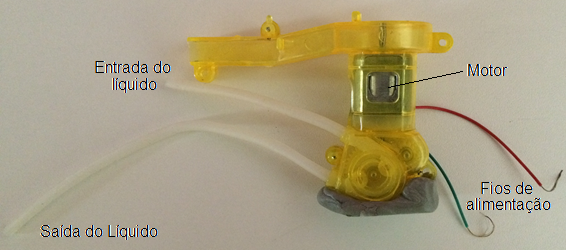
\includegraphics[scale=1.0]{figuras/bomba.png}
		\caption{Bomba peristáltica utilizada no projeto}
		\label{bomba}
\end{figure}

Outro pré-requisito que a bomba deve atender para ser considerada apropriada para o projeto é ser capaz de fornecer a vazão apropriada de fluido para a limpeza da lente, considerando o tamanho da caixa na qual esta estará armazenada. Para isto, realizou-se um teste de vazão. Na figura \ref{esquematico} é possível visualizar o esquemático do teste e na figura \ref{proveta} a proveta utilizada no teste.

\begin{figure}[H]
		\centering
			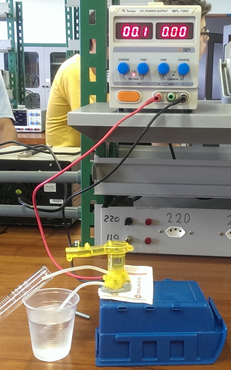
\includegraphics[scale=1.0]{figuras/esquematico.png}
		\caption{Esquemático do teste}
		\label{esquematico}
\end{figure}


\begin{figure}[H]
		\centering
			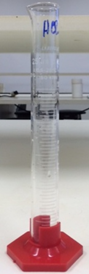
\includegraphics[scale=1.0]{figuras/proveta.png}
		\caption{Proveta utilizada no teste}
		\label{proveta}
\end{figure}


Para o teste, utilizou-se uma fonte de tensão, a bomba peristáltica, um suporte para a bomba, um recipiente com água e uma proveta graduada. Ajustou-se a fonte de tensão para diferentes valores e a bomba funcionou pelo período de 1 minuto, retirando água do recipiente e despejando-a na proveta. Após o tempo determinado, observou-se na proveta o quanto de água foi movimentada, registrando-se o valor. Segue na figura \ref{resultadosbomba} os valores obtidos.

\begin{figure}[H]
		\centering
			\includegraphics[scale=1.0]{figuras/resultadosbomba.png}
		\caption{Resultados do teste}
		\label{resultadosbomba}
\end{figure}


A quantidade de fluido utilizada para limpeza da lente está estimada em 4 mililitros, portanto, a bomba peristáltica testada prova-se suficiente para a função pretendida.






\section[Sistema de Sucção]{Sistema de Sucção}

O sistema de sucção será responsável por gerar a pressão negativa necessária para manter a lente na posição correta no momento em que esta for ser removida da caixa de lente. Este sistema será composto por: uma seringa graduada, equipo hospitalar (tubos plásticos) e um servo motor. 

Ao arranjar os componentes citados de forma adequada é possível fazer com que utilizando a lei dos gases ideais $PV= NRT$ a pressão ($P$) dentro do tubo varie de acordo com a variação do volume de ar dentro da seringa ($V$). Assim sendo, considerando o processo isotérmico e que não há fugas de gás atmosférico para dentro dos tubos é possível que a seguinte equação seja aplicada:


\begin{center}
$P_i \cdot V_i = P_f \cdot V_f$
\end{center}

Ou seja, a variação de pressão dentro do tubo é proporcional à variação do volume do ar que ocupa o espaço. Assim sendo quando utilizando o servo motor o embolo da seringa for deslocado de forma a aumentar o volume total do sistema, a pressão desse sistema irá cair proporcionalmente à essa variação deste volume e assim a pressão atmosférica irá empurrar a lente para dentro do tubo. Deixando assim a lente fixa na saída do tubo, o qual terá a forma da concavidade de um olho.

Esse sistema foi inicialmente imaginado para além de manter a lente na posição correta dentro da caixa de lente, para também transportar a lente da caixa de lentes até o olho do usuário, assim como o caminho inverso.  Porém outra solução para o transporte da lente foi encontrada e o sistema de sucção foi substituído nesta tarefa, ficando a cargo deste sistema somente manter a lente na posição correta dentro da caixa de lente.


\subsection[Ensaios]{Ensaios}

Foram realizados dois ensaios para este sistema. Estes ensaios tinham como objetivo principal observar se existia necessidade de se utilizar este sistema na caixa de lente. Para tal foram confeccionadas duas caixas para a lente, feitas de papelão e isopor, uma vez que a caixa fabricada na impressora 3D não estava pronta. Neste teste foram utilizadas duas calotas esféricas obtidas a partir de uma pequena bolinha de borracha de 3$cm$ de diâmetro para simular o apoio da lente na caixinha de forma a se aproximar ao máximo do desenho real da caixa da lente. 

No primeiro teste as calotas esféricas não continham os furos para passar os tubos do sistema de sucção. O teste foi o seguinte: posicionar a lente sobre a calota, encher lentamente a caixinha com água até que as lentes estivessem cobertas de água e em seguida inclinar em $90^\circ$ a caixa para observar como as lentes se comportam. O teste foi realizado vinte vezes. Em quatorze deles, as lentes permaneceram na posição correta, ou seja, mantiveram-se fixa juntamente com o apoio de borracha. Nas outras 6 vezes ao menos uma das lentes deslocou-se do apoio e escoou juntamente com a água para fora da caixinha de lente.

O segundo ensaio foi basicamente a repetição do primeiro ensaio utilizando o sistema de sucção.  Para tal as caixinhas de papelão e isopor utilizadas anteriormente foram modificadas de forma a encaixar os tubos do sistema de sucção. E novamente vinte vezes o mesmo roteiro anterior foi realizado, porém antes de inclinar a caixa a seringa foi deslocada em 5$ml$. Desta vez em nenhuma das repetições as lentes saíram da posição em que deveriam se encontrar.

Isto mostra a necessidade do sistema de sucção no recipiente das lentes para sempre garantir que elas estarão lá no momento da operação.





\section[Sistema de Alimentação]{Sistema de Alimentação}

O sistema de alimentação tem como objetivo prover um sistema de alimentação de corrente continua seguro que atenda às necessidades energéticas do produto e aos padrões de segurança exigidos pelas normas ABNT para produtos energizados (Fig. \ref{fig27}).

Utilizando materiais e equipamentos adequados, o sistema deve prover uma fonte continua e segura de energia elétrica. Além de que mesmo quando a rede básica de energia não esteja disponível o sistema deve prover a energia à partir de uma bateria e realizar essa comutação, entre a bateria e a rede básica, de forma automática e segura para os equipamentos elétricos e ao usuário.

O sistema será basicamente composto por uma fonte AC / DC, um controlador de carga de bateria, uma bateria eu uma placa com relês comutadores. A fonte  AC/DC , ligada diretamente na  rede elétrica 220V alternado irá prover uma carga 12-14V contínuos e este alimentará o controlador de carga. O controlador de carga é capaz de regular os níveis de tensão da bateria garantindo que quando esta estiver totalmente carregada a alimentação DC seja interrompida.

A placa de relês comutadores tem o objetivo isolar o equipamento quando este estiver realizando alguma manobra. Desta forma o sistema é capaz de prover o isolamento necessário da rede elétrica 220V AC. Sendo assim o equipamento não será perturbado com quais quer eventualidades, como um pico de corrente provado por uma descarga atmosférica ou eventual queda da rede 220V AC que possa vir a acontecer durante uma manobra. 


\textbf{Especificações:}

\textbf{Controlador de carga}
\begin{itemize}	
\item Tensão: 12V ou 24V DC(detecção automática);
\item Tensão da fonte de alimentação: 12.6V ou 25.2V DC;
\end{itemize}

\textbf{Fonte AC/DC}
\begin{itemize}
\item Tensão entrada: 220V AC;
\item Tensão saída: 14V DC;
\item Corrente saída: 500 mA;
\end{itemize}

\textbf{Bateria}
\begin{itemize}
\item Tensao de Carga: 13,8V;
\item Tensao de Descarga: 12V;
\item Capacidade de carga: 1Ah;
\end{itemize}

\textbf{Placo Comutadora}
\begin{itemize}
\item Tensao de Carga: 24 VDC;
\item Tensao de Descarga: 7A;
\item Capacidade de carga: 5 V DC;
\end{itemize}

\begin{figure}[H]
		\centering
			\includegraphics[scale= 0.7]{figuras/alimentacao.png}
		\caption{Sistema de Alimentação}
		\label{fig27}
\end{figure}